
\section{Detección no coherente}

Supongamos que no tengo la información de fase de la portadora
(pero sí tengo sincronismo a nivel de símbolos). $x_c(t)=a_k
p(t-kT_s)\cos(\omega_ct+\theta)$ donde $p(t)$ es un pulso
rectangular.

Si pongo un filtro apareado, a menos de $\theta$: $h(t) = \cos(\omega_ct)p(t)$ (desconoce $\theta$) pasabanda, me sale algo así:

%\begin{figure}[h]
%    \centering
\begin{center}\begin{minipage}{\textwidth}
    \bpgf{Imagenes/DDPasa/DDPasa-18}
    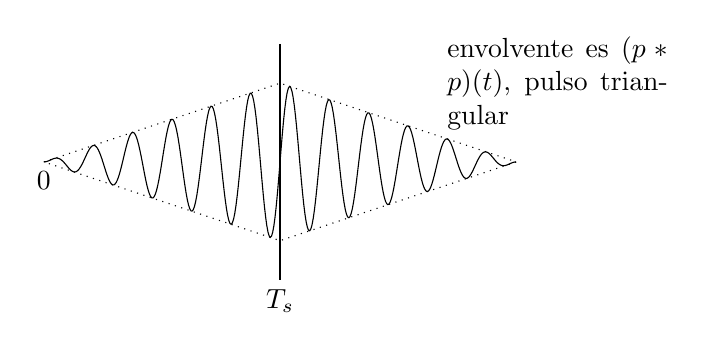
\begin{tikzpicture}
        \draw [dotted] (0,0) node [anchor=north] {$0$} -- (3,1) -- (6,0) -- (3,-1) -- (0,0);
        \draw [samples=200,domain=0:3] plot (\x,{\x/3*sin(4*pi*\x r)});
        \draw [samples=200,domain=3:6] plot (\x,{(6-\x)/3*sin(4*pi*\x r)});
        \draw (3,1.5) -- (3,-1.5) node [anchor=north] {$T_s$};
        \path (5,1) node [anchor=west] {\parbox[b]{2.8cm}{envolvente es $(p\ast p)(t)$, pulso triangular}};
    \end{tikzpicture}
    \endpgfgraphicnamed\end{minipage}
\end{center}
%\end{figure}

Si el filtro tuviese la fase correcta, muestreando en $T_s$ tengo la detección óptima. Pero, dado el error de fase $\theta$, la oscilación no tiene por qué llegar al máximo en $t=T_s$. Si muestreo ahí, me da cualquier cosa.

\paragraph{Solución} Tomar la envolvente.

\begin{figure}[htb]
    \centering
    \bpgf{Imagenes/DDPasa/DDPasa-19}
    \begin{blockdiagram}
        \matrix[row sep=5mm,column sep=10mm]{
            & \node [punto] (p) {};\\
            \node [etiqueta] (inicio) {$a_k p(t-kT_s)\cos(\omega_c t+\theta)$}; & \node[operator] (sum) {$+$}; & \node[block] (filtro) {$h(t)$}; & \node [block] (det) {DET. ENV.};& \node [block] (delim) {COMP.};\\
        };
        \draw [->] (inicio) -- (sum);
        \draw [->] (p) -- (sum);
        \draw [->] (sum) -- (filtro);
        \draw [->] (filtro) -- (det);
        \draw [->] (det) -- (delim);
    \end{blockdiagram}
    \endpgfgraphicnamed
\end{figure}

\begin{itemize}
    \item Esto sirve para ASK, pero no para PSK (ni siquiera BPSK) ya que cambia la fase, no altera la envolvente
    \item Se puede usar para FSK

    \begin{center}
        \resizebox{0.8\textwidth}{!}{
        \bpgf{Imagenes/DDPasa/DDPasa-20}
        \begin{blockdiagram}
            \matrix[row sep=5mm,column sep=10mm,ampersand replacement=\&]{
                \& \& \node[block] (pasa1) {PASA: $[f_c,f_c+\frac{\Delta f}{2}]$}; \& \node [block] (det1) {DET. ENV.};\\
                \node [etiqueta] (inicio) {$x_c(t)$}; \& \node [punto] (p) {}; \& \& \& \node [operator] (sum) {} node [anchor=north east] {$-$} node [anchor=south east] {$+$};\& \node [block] (comp) {COMP.};\\
                \& \& \node[block] (pasa2) {PASA: $[f_c-\frac{\Delta f}{2},f_c]$}; \& \node [block] (det2) {DET. ENV.};\\
            };
            \draw (inicio) -- (p);
            \draw [->] (p) |- (pasa1);
            \draw [->] (pasa1) -- (det1);
            \draw [->]  (det1) -| (sum);
            \draw [->] (p) |- (pasa2);
            \draw [->] (pasa2) -- (det2);
            \draw [->]  (det2) -| (sum);
            \draw [->] (sum) -- (comp);
        \end{blockdiagram}
        \endpgfgraphicnamed}
    \end{center}

    Aunque las bandas no estén separadas del todo, da más fuerte la señal correcta.
\end{itemize}

\subsubsection*{PSK diferencial (DPSK)}

Una forma de hacer un detector no coherente para PSK es detectar
diferencias de fase con el símbolo anterior.

%\begin{figure}[h]
%    \centering
\begin{center}
   \resizebox{\textwidth}{!}{
    \bpgf{Imagenes/DDPasa/DDPasa-21}
    \begin{blockdiagram}
        \matrix[row sep=5mm,column sep=10mm,ampersand replacement=\&]{
            \node [etiqueta] (inicio) {$x_c(t)$}; \& \node[block] (pasa1) {PASABANDA}; \& \node [punto] (p) {}; \& \&\node [operator] (mult) {$\times$}; \& \node [block] (pasa2) {PASABAJOS}; \& \node[block] (comp) {COMP};\\
            \& \& \& \node [block] (ret) {Retardo $T_s$};\\
        };
        \draw [->] (inicio) -- (pasa1);
        \draw [->] (pasa1) -- (p) -- (mult);
        \draw [->] (p) |- (ret);
        \draw [->] (ret) -| (mult);
        \draw [->] (mult) -- (pasa2);
        \draw [->] (pasa2) -- (comp);
    \end{blockdiagram}
    \endpgfgraphicnamed}
\end{center}
%\end{figure}

Correlaciono un pulso de RF con el anterior. Si tienen la misma
fase, da mayor que $0$; si tienen fase opuesta, da menor que $0$.
Entonces el sistema detecta cambios en bits, no bits individuales.
Precodificando los bits transmito la información.
